\documentclass{beamer}
\usepackage[utf8]{inputenc}
\usepackage[T1]{fontenc}
\usepackage[swedish,english]{babel}
\usepackage{color}
\usepackage{xcolor}
\usepackage{amssymb}
\usepackage{amsmath}
\usepackage{ae}
\usepackage{units}
\definecolor{olive}{RGB}{0,139,69}
\usetheme{Pittsburgh}
\usecolortheme[RGB={0,139,69}]{structure}
\setbeamertemplate{navigation symbols}{}

\begin{document}

\section{Presentation}

\frame{
  \begin{center}

    \textcolor{olive}{{
        \Large Väderparametrars inverkan på \\ energiförluster i en fastighet
      } \\
      - en studie av värmeflöden
    }

    \vskip10pt

    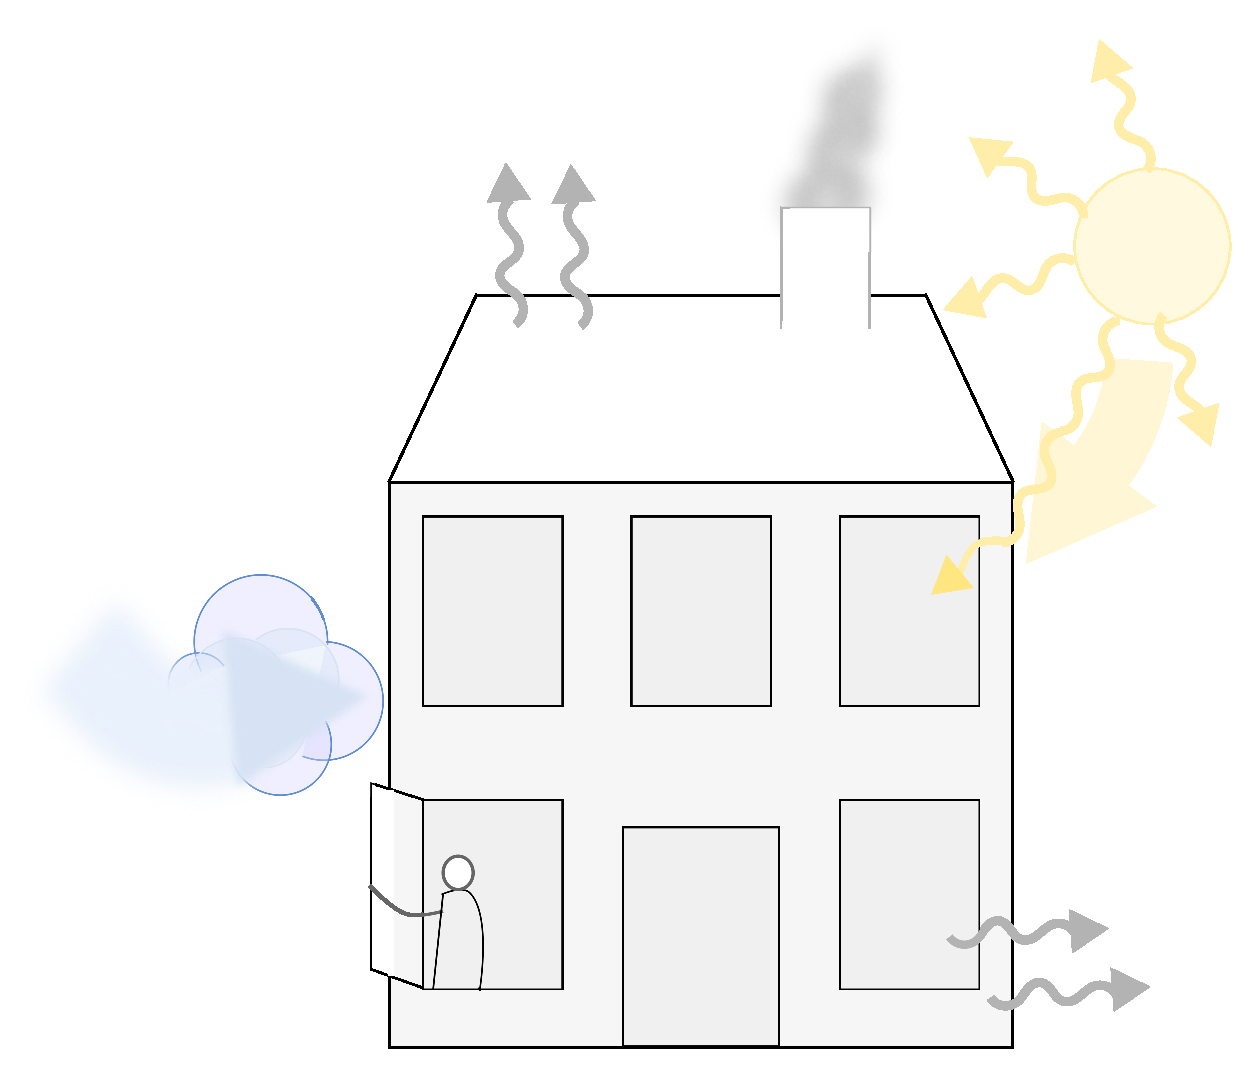
\includegraphics[scale=0.2]{../report/images/hus_framsida.eps}

    \vskip10pt

    Erik Ahlqvist, Ylva Dahl, Mats Lindström, Dan Ståby

    Institutionen för Teknisk Fysik

    29 maj, 2012

  \end{center}

}

\subsection{Byggnadsskal - väggar och tak}

%Definition av h-värde och U-värde

\frame{
       \frametitle{Några definitioner}
        \begin{align*}
        Q &= U\Delta T \\
        Q &= h(T-T_\infty)
        \end{align*}
        \begin{center}
          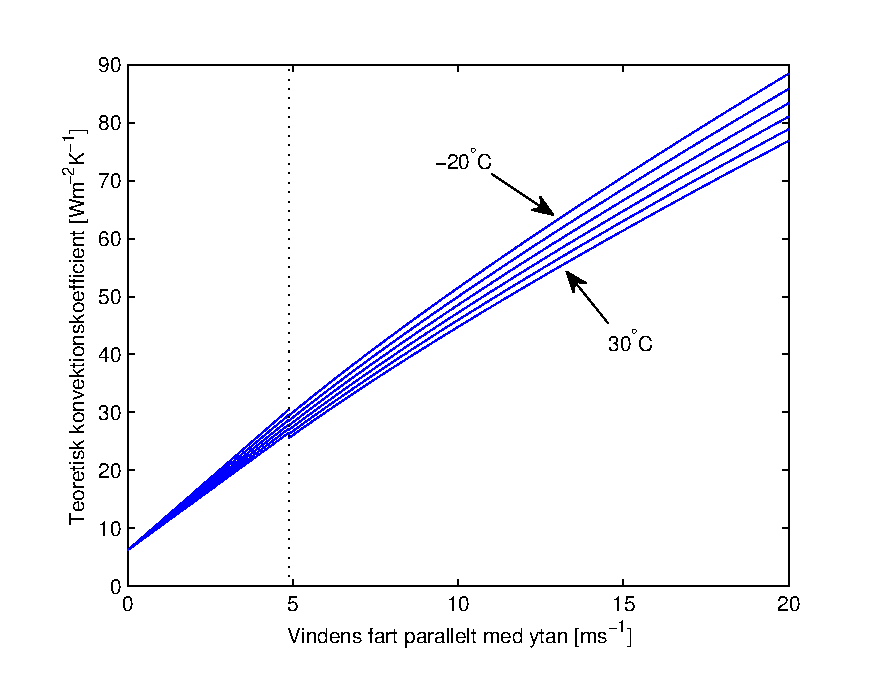
\includegraphics[scale=0.5]{../report/images/hvalues.eps}
        \end{center}
}


%Data för huset

\frame{
       \frametitle{Parametrar för huset}
        \begin{table}[hbtp]
        \centering
        \caption{Areor och U-värden för fastighetens klimatsköld. \emph{\color{red} Byta ut denna mot en mer talande figur?}}
        \label{tbl:uvalue}

        \begin{tabular}{|l|r|r|}
        \hline
        \textbf{Del} & \textbf{Area~$[\unit{m^2}]$} &\textbf{U-värde~$[\unit{W~m^{-2}~K^{-1}}]$} \\
        \hline
        Söderväggen &  151 & 1,186 \\ 
        Västerväggen & 61 & 1,186 \\
        Norrväggen & 290 & 0,279 \\
        Burspråket & 47 & 0,393 \\
        Taket & 257 & 0,171 \\
        \hline
        Fönster, söder & 109 & 1,0 \\
        Fönster, norr & 89 & 1,0 \\
        Fönster, tak & 8 & 1,0 \\
        \hline
        \textbf{Totalt} & \textbf{1012} & \textbf{0,6}\\
        \hline
        \end{tabular}
        \end{table}

}

\begin{frame}{Resultat}
 
\begin{figure}
        \begin{subfigure}[b]{0.48\textwidth}
                \centering
                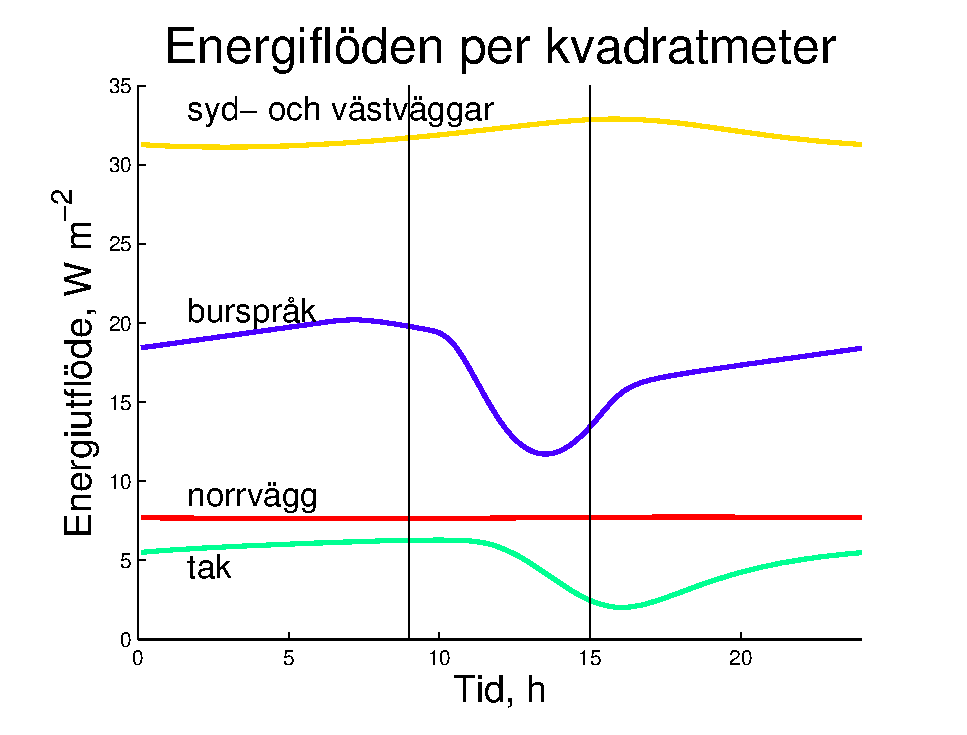
\includegraphics[width=\textwidth]{images/walls1.eps}
        \end{subfigure}
        \begin{subfigure}[b]{0.48\textwidth}
                \centering
                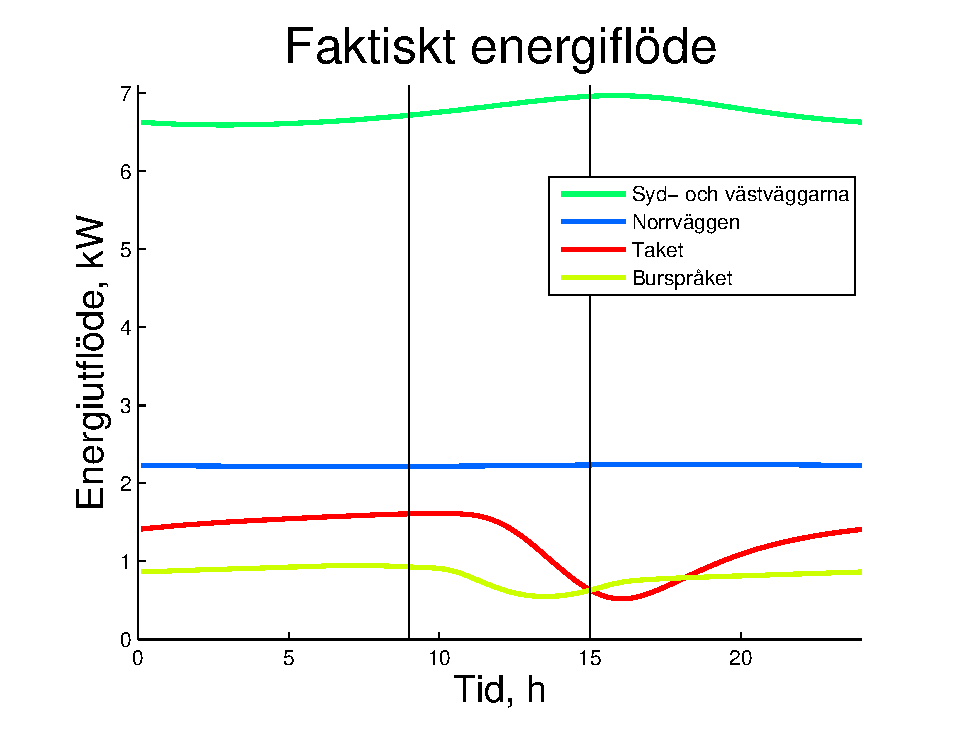
\includegraphics[width=\textwidth]{images/walls2.eps}
        \end{subfigure}
\end{figure}


\end{frame}



\end{document}
